\boxde
\Opensolutionfile{ans}[ans/2D1-2-DEON-1]
\begin{ex}%[2D1Y2-2]
    Cho hàm số $y=f(x)$ có bảng biến thiên như hình vẽ. Hàm số đã cho có bao nhiêu cực trị?
    \begin{center}
        
\begin{tikzpicture}[>=stealth]
            \tkzTabInit[nocadre=false,lgt=1,espcl=4,deltacl=0.5]{$x$/.6 ,$y'$/.6,$y$/1.6}
            {$-\infty$ , $1$ , $+\infty$}
            \tkzTabLine{ , - , d , - , }
            \tkzTabVar{+/$2$ , -D+/$-\infty$/$+\infty$ , -/$2$}
        \end{tikzpicture}
    \end{center}
    \choice
    {$2$}
    {$1$}
    {$3$}
    {\True $0$}
    \loigiai{Từ bảng biến thiên, hàm số đã cho không có cực trị.}
\end{ex}
\begin{ex}%[2D1Y2-2]
    Cho hàm số $y=f(x)$ có bảng biến thiên như sau.
    \begin{center}
        
\begin{tikzpicture}[>=stealth]
            \tkzTabInit[nocadre=false,lgt=1,espcl=2.7,deltacl=0.5]{$x$/.6 ,$y'$/.6,$y$/1.6}
            {$-\infty$ , $0$ , $3$ , $+\infty$}
            \tkzTabLine{ , - , $0$ , + , d , - , }
            \tkzTabVar{+/$8$ , -/$1$ , +/$4$ , -/$2$}
        \end{tikzpicture}
    \end{center}
    Hàm số đã cho có bao nhiêu cực trị?
    \choice
    {\True $2$}
    {$1$}
    {$3$}
    {$4$}
    \loigiai{Từ bảng biến thiên, hàm số đã cho đạt cực đại tại $x=3$ và đạt cực tiểu tại $x=0$, do đó hàm số có hai cực trị.}
\end{ex}

\begin{ex}%[2D1Y2-2]
    Cho hàm số có bảng biến thiên như hình vẽ.
    \begin{center}
        
\begin{tikzpicture}
            \tkzTabInit[espcl=2.7,lgt=1]
            {$x$/0.6,$y'$/0.6,$y$/1.6}
            {$-\infty$,$-1$,$2$,$+\infty$}
            \tkzTabLine{,+,0,-,0,+,}
            \tkzTabVar{-/$-\infty$,+/$4$,-/$-5$,+/$+\infty$}
        \end{tikzpicture}
    \end{center}
    Mệnh đề nào dưới đây \textbf{đúng}?
    \choice
    {Hàm số có bốn điểm cực trị}
    {\True Hàm số đạt cực tiểu tại $x=2$}
    {Hàm số không có cực đại}
    {Hàm số đạt cực tiểu tại $x=-5$}
    \loigiai{
        Dựa vào bảng biến thiên ta có hàm số đạt cực tiểu tại $ x=2 $.
    }
\end{ex}
\begin{ex}%[2D1Y2-2]
    Cho hàm số $y=f(x)$ có bảng biến thiên như hình vẽ.
    \begin{center}
        
\begin{tikzpicture}
            \tkzTabInit[espcl=2.5,lgt=1.5]
            {$x$/0.6,$y'$/0.6,$y$/1.6}
            {$-\infty$,$-2$,$-2$,$+\infty$}
            \tkzTabLine{,+,0,-,0,+,}
            \tkzTabVar{-/$-\infty$,+/$3$,-/$0$,+/$+\infty$}
        \end{tikzpicture}
    \end{center}
    Giá trị cực đại của hàm số đã cho bằng
    \choice
    {\True $ 3 $}
    {$ -2 $ }
    {$ 2 $ }
    {$ 0 $ }
    \loigiai{
        Từ bảng biến thiên ta tìm được giá trị cực đại của hàm số bằng $ 3 $.
    }
\end{ex}
\begin{ex}%[2D1Y2-2]
    Cho hàm số $f(x)$ liên tục trên $\mathbb{R}$ và có bảng biến thiên như hình vẽ.
    \begin{center}

        
\begin{tikzpicture}
            \tkzTabInit[espcl=2,lgt=1]
            {$x$/0.6,$y'$/0.6,$y$/2.2}
            {$-\infty$,$ -1 $,$ 2 $,$5$,$+\infty$}
            \tkzTabLine{,-,0,+,d,-,0,-,}
            \tkzTabVar{+/$+\infty$,-/$ -1 $,+/$ 3 $,R/,-/$-\infty$}
            \tkzTabVal{3}{5}{0.5}{}{$1$}
        \end{tikzpicture}
    \end{center}
    Khẳng định nào sau đây \textbf{đúng}?
    \choice
    {Hàm số có $ 1 $ cực đại và $ 2 $ cực tiểu}
    {\True Hàm số có $ 1 $ cực đại và $ 1 $ cực tiểu}
    {Hàm số có đúng $ 1 $ cực trị}
    {Hàm số có $ 2 $ cực đại và $ 1 $ cực tiểu}
    \loigiai{
        Dựa vào bảng biên thiên ta được  hàm số có $ 1 $ cực đại và $ 1 $ cực tiểu.
    }
\end{ex}
%%==========Câu 47
\begin{ex}%[2D1B2-2]
    Cho hàm số $y=f(x)$ liên tục trên $[a;b]$ và có đồ thị như hình vẽ bên. Số điểm cực tiểu của hàm số đã cho là
    \begin{center}
        \begin{tikzpicture}[>=stealth,line join=round, line cap=round, font=\footnotesize,scale=0.7]
            \draw[-stealth](-4,0)--(0,0)node[below left]{$O$}--(4,0)node[below left]{$x$};
            \draw[-stealth](0,-2)--(0,3)node[below left]{$y$};
            \draw[dashed]
            (-3,0)node[below]{$a$}--(-3,2)
            (3,0)node[above]{$b$}--(3,-1.5)
            ;
            \draw[smooth]
            (-3,2)..controls+(-75:2) and+(180:.5)..(-2,-1)
            ..controls+(0:.5) and+(180:.5)..(-.75,1)
            ..controls+(0:.5)and+(120:.5)..(0,0)
            ..controls+(-60:.5)and+(180:.25)..(0.75,-.75)
            ..controls+(0:.5)and+(180:.3)..(1.75,2)
            ..controls+(0:.5)and+(110:.3)..(3,-1.5)
            ;
        \end{tikzpicture}
    \end{center}
    \choice
    {$6$}
    {$4$}
    {$3$}
    {\True $2$}
    \loigiai{
        Dựa vào đồ thị ta thấy hàm số đã cho có $2$ điểm cực tiểu.
    }
\end{ex}
%%==========Câu 56
\begin{ex}%[2D1K2-2]
    Cho hàm số $y=f(x)$ có đồ thị như hình vẽ bên. Đường thẳng đi qua hai điểm cực tiểu của đồ thị hàm số đã cho có phương trình.
    \begin{center}
        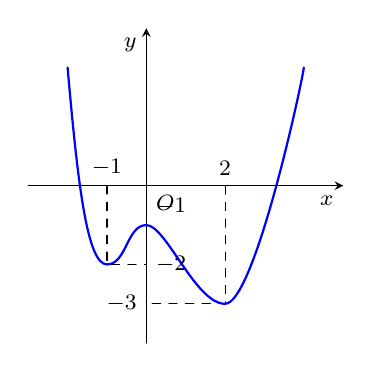
\begin{tikzpicture}[>=stealth,line join=round, line cap=round, font=\footnotesize,scale=0.5]
            \draw[-stealth](-3,0)--(0,0)node[below right]{$O$}--(5,0)node[below left]{$x$};
            \draw[-stealth](0,-4)--(0,-1)node[above right]{$-1$}--(0,4)node[below left]{$y$};
            \draw[dashed]
            (-1,0)node[above]{$-1$}|-(0,-2)node[right]{$-2$}
            (2,0)node[above]{$2$}|-(0,-3)node[left]{$-3$}
            ;
            \draw[smooth,thick,blue]
            (-2,3)..controls+(-85:3) and+(180:.5)..(-1,-2)
            ..controls+(0:.5)and+(180:.5)..(0,-1)
            ..controls+(0:.5)and+(180:.75)..(2,-3)
            ..controls+(0:.75)and+(-95:.3)..(4,3)
            ;
        \end{tikzpicture}
    \end{center}
    \choice
    {$y=-5x-7$}
    {\True $y=-\dfrac{1}{3}x-\dfrac{7}{3}$}
    {$y=-5x+7$}
    {$y=-\dfrac{1}{3}x+\dfrac{7}{3}$}
    \loigiai{
        Gọi $A(-1;-2)$ và $B(2;-3)$ là 2 điểm cực tiểu của đồ thị hàm số đã cho.\\
        Giả sử đường thẳng đi qua $A$ và $B$ có phương trình $\Delta\colon y=ax+b$.\\
        Ta có hệ phương trình $\heva{&-a+b=-2\\&2a+b=-3.}\Leftrightarrow \heva{&a=-\dfrac{1}{3}\\&b=-\dfrac{7}{3}.}$.\\Vậy $\Delta \colon y=-\dfrac{1}{3}x-\dfrac{7}{3}.$
    }
\end{ex}
\begin{ex}%[2D1B2-2]
    Cho hàm số $y=f(x)$ có bảng biến thiên như hình vẽ.
    \begin{center}
        
\begin{tikzpicture}
            \tkzTabInit[espcl=2.5,lgt=1]
            {$x$/0.6,$y'$/0.6,$y$/1.7}
            {$-\infty$,$0$,$2$,$+\infty$}
            \tkzTabLine{,-,0,+,0,-,}
            \tkzTabVar{+/$+\infty$,-/$1$,+/$5$,-/$-\infty$}
        \end{tikzpicture}
    \end{center}
    Khoảng cách giữa hai điểm cực trị của đồ thị hàm số đã cho bằng
    \choice
    {\True $2 \sqrt{5}$}
    {$\sqrt{10}$}
    {$\sqrt{5}$}
    {$2 \sqrt{3}$}
    \loigiai{
        Từ bảng biến thiên ta được điểm cực tiểu của đồ thị hàm số là $ (0;1) $. Điểm cực đại của đồ thị hàm số là $ (2;5) $. Khi đó khoảng cách hai điểm cực trị là \[ \sqrt{(0-2)^2+(1-5)^2}=2\sqrt{5}. \]
    }
\end{ex}
\begin{ex}%[2D1B2-2]
    Cho hàm số $y=f(x)$ liên tục trên $\mathbb{R}$ và có bảng biến thiên như hình vẽ.
    \begin{center}
        
\begin{tikzpicture}
            \tkzTabInit[espcl=2.5,lgt=1]
            {$x$/0.6,$y'$/0.6,$y$/2}
            {$-\infty$,$1$,$2$,$+\infty$}
            \tkzTabLine{,+,d,-,d,+,}
            \tkzTabVar{-/$-4$,+/$3$,-/$-5$,+/$+\infty$}
        \end{tikzpicture}
    \end{center}
    Đường thẳng đi qua hai điểm cực trị của đồ thị hàm số đã cho có phương trình
    \choice
    {$y=-8 x-11$}
    {$y=8 x+11$}
    {$y=8 x-11$}
    {\True $y=-8 x+11$}
    \loigiai{
        Hai điểm cực trị của đồ thị hàm số là $ (1;3) $ và $ (2;-5) $. Đường thẳng qua hai điểm cực trị có dạng $ y=ax+b $ nên ta có \[ \heva{&3=a \cdot 1+b\\&-5=a \cdot 2+b } \Leftrightarrow \heva{&a=-8\\&b=11} \Rightarrow y=-8x+11. \]
    }
\end{ex}
\begin{ex}%[2D1B2-1]
    Hàm số $y=\dfrac{2x+3}{x+1}$ có bao nhiêu cực trị
    \choice
    {$3$}
    {\True $0$}
    {$2$}
    {$1$}
    \loigiai{
        \begin{enumerate}[$ \star $]
            \item Tập xác định $\mathscr{D}=\mathbb{R}\setminus\left\{-1\right\}.$
            \item Đạo hàm $y'=\dfrac{-1}{(x+1)^2}<0,\forall x\in\mathscr{D}$.
            %	\item Tiệm cận đứng: $x=-1$, vì $\lim\limits_{x\to\left(-1\right)^-}y=-\infty$ và $\lim\limits_{x\to\left(-1\right)^+}y=+\infty$
            %	\item Tiệm cận ngang: $y=2$, vì $\lim\limits_{x\to\pm\infty}y=2$.
            \item Bảng biến thiên
            \begin{center}
                
\begin{tikzpicture}[>=stealth,line join=round, line cap=round, font=\footnotesize,scale=0.8]
                    \tkzTabInit[nocadre=false,lgt=1.2,espcl=2.5,deltacl=0.6]
                    {$x$/0.6,$y'$/0.6,$y$/2}
                    {$-\infty$,$-1$,$+\infty$}
                    \tkzTabLine{,-,d,-,}
                    \tkzTabVar{+/$2$,-D+/$-\infty$/$+\infty$,-/$2$}
                \end{tikzpicture}
            \end{center}
            %	\item Hàm số nghịch biến trên từng khoảng xác định.
            \item Hàm số không có cực trị.
        \end{enumerate}
    }
\end{ex}
\begin{ex}%[2D1B2-1]
    Cho hàm số $y=\sqrt{x^2-x-20}$. Mệnh đề nào sau đây \textbf{sai}?
    \choice
    {Hàm số nghịch biến trên khoảng $(-\infty;-4)$}
    {Hàm số đạt cực đại tại $x=5$}
    {\True Hàm số đồng biến trên khoảng $(5;+\infty)$}
    {Hàm số không có cực trị}
    \loigiai
    {
        Tập xác định của hàm số $\mathscr{D}=(-\infty;-4]\cup[5;+\infty)$. Ta có $y'=\dfrac{2x-1}{2\sqrt{x^2-x-20}}$.\\
        Với $y'=0\Leftrightarrow \dfrac{2x-1}{2\sqrt{x^2-x-20}}=0\Leftrightarrow x=\dfrac{1}{2}\not\in\mathscr{D}$.\\
        Bảng xét dấu của $y'$ như hình dưới.
        \begin{center}
            
\begin{tikzpicture}
                \tkzTabInit[nocadre=false,lgt=1.2,espcl=2.5,deltacl=0.6]
                {$x$/1, $y'$/1}
                {$-\infty$, $-4$, $5$, $+\infty$}
                \tkzTabLine{,-,,h,,+,}
            \end{tikzpicture}
        \end{center}
        Ta thấy trong khoảng $(5;+\infty)$ thì $y'>0$ nên hàm số đồng biến trên khoảng $(5;+\infty)$.
    }
\end{ex}


\begin{ex}%[2D1B2-1]
    Hàm số nào trong bốn hàm số được liệt kê dưới đây không có cực trị?
    \choice
    {\True $y=\dfrac{2x-1}{x+1}$}
    {$y=x^4$}
    {$y=-x^3+x$}
    {$ y=|x|$}
    \loigiai{
        Xét hàm số $y=\dfrac{2x-1}{x+1}$ ta có $y'=\dfrac{3}{(x+1)^2}> 0$ với $x\neq-1$ nên hàm số không có cực trị.}
\end{ex}


\begin{ex}%[2D1B2-1]
    Điểm cực tiểu của hàm số $y=x^3-3x^2-9x+2$ là
    \choice
    {$x=11$}
    {\True $x=3$}
    {$x=7$}
    {$x=-1$}
    \loigiai{
        Ta có $y'=3x^2-6x-9$.\\
        $y'=0 \Leftrightarrow 3x^2-6x-9=0 \Leftrightarrow \hoac{&x=-1\\&x=3.}$\\
        Bảng biến thiên của hàm số
        \begin{center}
            
\begin{tikzpicture}
                \tkzTabInit[nocadre=false,lgt=1.2,espcl=2.5,deltacl=0.6]
                {$x$ /0.6,$y'$ /0.6,$y$ /2}
                {$-\infty$,$-1$,$3$,$+\infty$}
                \tkzTabLine{,+,$0$,-,$0$,+,}
                \tkzTabVar{-/$-\infty$,+/$7$,-/$-25$,+/$+\infty$}
            \end{tikzpicture}
        \end{center}
        Dựa vào bảng biến thiên, hàm số đạt cực tiểu tại $x=3$.
    }
\end{ex}
%%==========Câu 45
\begin{ex}%[2D1B2-1]
    Với giá trị thực nào của tham số $m$ để đường thẳng $y=(3m+1)x+3+m$ vuông góc với đường thẳng đi qua hai điểm cực trị của đồ thị hàm số $y=x^3-3x^2-1$?
    \choice
    {$m=\dfrac{1}{6}$}
    {$m=-\dfrac{1}{3}$}
    {\True $m=-\dfrac{1}{6}$}
    {$m=\dfrac{1}{3}$}
    \loigiai{
        \begin{enumerate}[$ \star $]
            \item Tập xác định $\mathscr{D}=\mathbb{R}.$
            \item Đạo hàm $y'=3x^2-6x$.
            \item $y'=0\Leftrightarrow \hoac{&x=0\Rightarrow y=-1\\&x=2\Rightarrow y=-5}$
            %	\item Giới hạn $\lim\limits_{x\to-\infty}y=-\infty$, $\lim\limits_{x\to+\infty}y=+\infty$.
            \item Bảng biến thiên
            \begin{center}
                
\begin{tikzpicture}[>=stealth,line join=round, line cap=round, font=\footnotesize,scale=0.8]
                    \tkzTabInit[nocadre=false,lgt=1.2,espcl=2.5,deltacl=0.6]
                    {$x$/0.6,$y'$/0.6,$y$/2}
                    {$-\infty$,$0$,$2$,$+\infty$}
                    \tkzTabLine{,+,0,-,0,+,}
                    \tkzTabVar{-/$-\infty$,+/$-1$,-/$-5$,+/$+\infty$}
                \end{tikzpicture}
            \end{center}
            \item Hàm số đạt cực đại tại $x=0$, $y_{\textrm{CĐ}}=-1$.
            \item Hàm số đạt cực tiểu tại $x=2$, $y_{\textrm{CT}}=-5$.
            \item Đường thẳng đi qua hai cực trị có dạng $y=ax+b$.\\
            Ta có $\heva{&b=-1\\&2a+b=-5}\Leftrightarrow \heva{&a=-2\\&b=-1.}$\\
            Do đó $y=-2x-1$ vuông góc với đường thẳng $d\colon y=(3m+1)x+3+m$ khi và chỉ khi \[(3m+1)\cdot(-2)=-1\Leftrightarrow m=-\dfrac{1}{6}.\]
        \end{enumerate}
    }
\end{ex}
\begin{ex}%[2D1K2-1]
    Cho hàm số $y=f(x)$ liên tục trên $\mathbb{R}$, có đạo hàm $f'(x)=(x-1)(x^2-2)(x^4-4)$. Số điểm cực trị của hàm số $y=f(x)$ là
    \choice
    {\True $1$}
    {$2$}
    {$4$}
    {$3$}
    \loigiai
    {
        Ta có $f'(x)=(x-1)(x^2-2)^2(x^2+2)$
        \begin{eqnarray*}
            f'(x)=0 \Leftrightarrow \hoac{&x-1=0 \\ &x^2-2=0} \Leftrightarrow \hoac{
                &x=1 \ (\text{Nghiệm đơn})\\
                &x=\pm \sqrt{2} \ (\text{Nghiệm bội chẵn}).
            }
        \end{eqnarray*}
        Suy ra hàm số chỉ có một cực trị.
    }
\end{ex}

\begin{ex}%[2D1Y2-2]
    \immini
    {
        Cho hàm số $f(x)$ có đạo hàm trên $\mathbb{R}$ và đồ thị hàm số $y=f'(x)$ trên $\mathbb{R}$ như hình vẽ. Mệnh đề nào đúng?
        \choice
        {\True Hàm số $y=f(x)$ có $1$ điểm cực đại và $1$ điểm cực tiểu}
        {Hàm số $y=f(x)$ có $2$ điểm cực đại và $2$ điểm cực tiểu}
        {Hàm số $y=f(x)$ có $1$ điểm cực đại và $2$ điểm cực tiểu}
        {Hàm số $y=f(x)$ có $2$ điểm cực đại và $1$ điểm cực tiểu}
    }
    {
        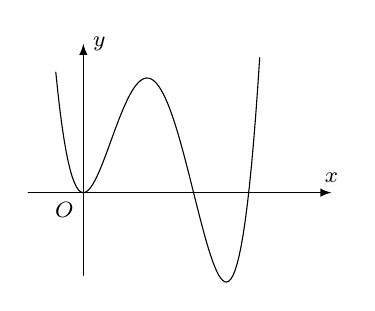
\begin{tikzpicture}[scale=0.7, font=\footnotesize, line join=round, line cap=round, >=stealth]
            \draw[->,>=latex](-1,0)--(4.5,0)node[above]{$x$};
            \draw[->,>=latex](0,-1.5)--(0,2.7)node[right]{$y$};
            \node[below left] at (0,0){$O$};
            \draw plot [samples=100,domain=-0.5:3.2] (\x,{((\x)^2)*(\x-2)*(\x-3)});
        \end{tikzpicture}
    }
    \loigiai
    {
        Ta thấy dấu của $f'(x)$ đổi dấu từ dương sang âm $1$ lần và từ âm sang dương $1$ lần.\\
        Do đó hàm số $f(x)$ có $1$ điểm cực đại và $1$ điểm cực tiểu.
    }
\end{ex}

\begin{ex}%[2D1B2-1]
    Tập hợp các giá trị của tham số thực $m$ để hàm số $y=x^4-2(m+2)x^2+3m-1$ chỉ có điểm cực tiểu, không có điểm cực đại là
    \choice
    {$(-\infty;-2)$}
    {$\{-2;2\}$}
    {$(-2;+\infty)$}
    {\True $(-\infty;-2]$}
    \loigiai{
        Hàm số đã cho chỉ có điểm cực tiểu mà không có điểm cực đại
        khi và chỉ khi
        $$1 \cdot (-2)(m+2)\ge 0\Leftrightarrow m\le -2.$$
    }
\end{ex}
\begin{ex}%[2D1B2-4]
    Tìm tất cả các giá trị của tham số $m$ để hàm số $y=\dfrac{1}{3}(m+1)x^3-x^2+(2m+1)x+3$ có cực trị.
    \choice
    {$m\in \left[ -\dfrac{3}{2};0 \right]$}
    {\True $m\in \left( -\dfrac{3}{2};0 \right) $}
    {$m\in \left( -\dfrac{3}{2};0 \right)\setminus \{-1\} $}
    {$m\in \left[ -\dfrac{3}{2};0 \right]\setminus \{-1\}$}
    \loigiai{
        \begin{itemize}
            \item Xét $m=-1$, ta có $y=-x^2-x+3$ là hàm bậc hai có đồ thị là đường parabol có một cực trị là đỉnh của parabol. Vậy $m=-1$ (nhận).
            \item Xét $m\ne -1$, ta có $y'=(m+1)x^2-2x+2m+1$.\\ Để hàm số có cực trị thì $$\left\{ \begin{aligned} &a\ne 0\\ &\Delta_{y'}>0 \end{aligned} \right.\Leftrightarrow \left\{ \begin{aligned} &m+1\ne 0\\ & 1-(m+1)(2m+1)>0 \end{aligned} \right.\Leftrightarrow \left\{ \begin{aligned} &m\ne -1\\ &-2m^2-3m>0 \end{aligned} \right.\Leftrightarrow \left\{ \begin{aligned} & m\ne -1\\ &-\dfrac{3}{2}<m<0.\end{aligned} \right.$$
        \end{itemize}
    }
\end{ex}
\begin{ex}%[2D1B2-4]
    Tìm $m$ để hàm số $y=mx^4+2(m-1)x^2+2$ ($m$ là tham số) có hai điểm cực tiểu và một điểm cực đại.
    \choice
    {\True $ 0<m<1 $}
    {$ 1<m<2 $}
    {$ m<0 $}
    {$ m>2 $}
    \loigiai{
        Hàm số có hai điểm cực tiểu và một điểm cực đại khi và chỉ khi $$\heva{&-\dfrac{b}{2a}>0\\ &a>0} \Leftrightarrow \heva{&-\dfrac{m-1}{m}>0\\ &m>0} \Leftrightarrow \heva{&0<m<1\\ &m>0} \Leftrightarrow 0<m<1.$$
    }
\end{ex}
\begin{ex}%[2D1B2-5]
    Cho hàm số $y=mx^4+2(m-1)x^2+6m-5$. Hàm số có đúng một cực trị khi và chỉ khi
    \choice
    {$\hoac{&m<0\\&m\ge 1}$}
    {$0\le m\le 1$}
    {$0<m<1$}
    {\True $\hoac{&m\le 0\\&m\ge 1}$}
    \loigiai{Xét $m=0$, hàm số trở thành $y=-2x^2+1$ có duy nhất một cực trị.\\
        Xét $m\ne 0$, khi đó hàm số có đúng một cực trị khi tích $a\cdot b\geq 0$ với $a, b$ là các hệ số của hàm bậc $4$ trùng phương. Hay $m(m-1)\ge0\Leftrightarrow\hoac{&m<0\\&m\ge1.}$\\
        Kết hợp với $m=0$, ta suy ra $\hoac{&m\le 0\\&m\ge1.}$
    }
\end{ex}
\begin{ex}%[2D1B2-3]
    Tìm tất cả các giá trị của $m$ để hàm số $f(x)=-x^3+2(2m-1)x^2-(m^2-8)x$ đạt cực tiểu tại điểm $x=-1$.
    \choice
    {$ m=-9 $}
    {$ m=-2 $}
    {\True $ m=1 $}
    {$ m=3 $}
    \loigiai{
        Ta có $\mathscr{D}=\mathbb{R}$.\\
        $y'=-3x^2+4(2m-1)x-m^2+8,\,y''=-6x+4(2m-1)$.\\
        Để $x=-1$ là điểm cực tiểu của hàm số khi $\heva{&y'(-1)=0\\&y''(-1)>0.}$\\
        Mà $y'(-1)=0\Leftrightarrow m^2+8m-9=0\Leftrightarrow\hoac{&m=1\\&m=-9.}$\\
        Với $m=1$ ta có $y''(-1)>0$ (nhận).\\
        Với $m=-9$ ta có $y''(-1)<0$ (loại).
    }
\end{ex}
\begin{ex}%[2D1B2-3]
    Cho hàm số $y=x^3-2x^2+ax+b$, ($a,b\in\mathbb{R}$) có đồ thị $(C)$. Biết đồ thị $(C)$ có điểm cực trị là $A(1;3)$. Tính giá trị của $P=7a+8b+84ab$.
    \choice
    {$P=282$}
    {$P=281$}
    {\True $P=283$}
    {$P=280$}
    \loigiai{
        Ta có $y'=3x^2-4x+a$.\\
        Đồ thị $(C)$ có điểm cực trị là $A(1;3)$ nên ta có $$\heva{&y'(1)=0 \\ &y(1)=3} \Leftrightarrow \heva{&a-1=0 \\ &a+b-1=3} \Leftrightarrow \heva{&a=1 \\ &b=3.}$$
        Khi đó $P=7a+8b+84ab=283$.
    }
\end{ex}
\begin{ex}%[2D1B2-3]
    Cho hàm số $y=\dfrac{1}{3}\sin 3x+m\sin x$. Tìm tất cả các giá trị của $m$ để hàm số đạt cực đại tại điểm $x=\dfrac{\pi}{3}$.
    \choice
    {$m=0$}
    {$m>0$}
    {$m=\dfrac{1}{2}$}
    {\True $m=2$}
    \loigiai{
        Ta có $y'=\cos 3x+m\cos x\Rightarrow y''=-3\sin 3x-m\sin x$.\\
        Hàm số đạt cực đại tại điểm $x=\dfrac{\pi}{3}$ với điều kiện cần $\Leftrightarrow\heva{&y'\left(\dfrac{\pi}{3}\right)=0\\&y''\left(\dfrac{\pi}{3}\right)<0}\Leftrightarrow\heva{&-1+\dfrac{1}{2}m=0\\&-\dfrac{\sqrt{3}}{2}m<0}\Leftrightarrow m=2$. \\
        Thử lại thấy $m=2$ thỏa mãn.
    }
\end{ex}
\begin{ex}%[2D1K2-4]
    Có bao nhiêu giá trị nguyên của tham số $m$ để  hàm số $y=  x^3  - 3 x   + 1 -m$ có  giá trị cực đại và giá trị cực tiểu trái dấu?
    \choice
    {$1$}
    {\True $3$}
    {$5$}
    {Vô số}
    \loigiai{
        Tập xác định $\mathscr{D} = \mathbb{R}$.\\
        $y'=3x^2 -3 =0\Leftrightarrow \hoac{&x=-1\\ &x=1.}$\\
        %Ta có $y''=6x$.\\
        %Tại $x_1=-1$, $y'(x_1) = 0$, $y''(x_1) =  -6<0$, suy ra điểm $M_1(-1;y(-1)= 3- m)$ là điểm    cực đại của đồ thị hàm số.\\
        %Tại $x_2=1$, $y'(x_2) = 0$, $y''(x_2) =   6>0$, suy ra điểm $M_2(1;y(1)=-m-1)$ là điểm    cực tiểu của đồ thị hàm số.\\
        Để  hàm số $y=  x^3  - 3 x   + 1 -m$ có  giá trị cực đại và giá trị cực tiểu trái dấu
        \[\Leftrightarrow y(-1)\cdot y(1)<0\Leftrightarrow (3-m)(-m-1)<0\Leftrightarrow -1<m<3.\]
        Vì $m\in \mathbb{Z}$ nên $m\in \{0;1;2\}$. Vậy có $3$ giá trị $m$ thỏa mãn yêu cầu bài toán.
    }
\end{ex}
\begin{ex}%[2D1B2-3]
    Cho hàm số $y=\dfrac{1}{3}x^3-m x^2+\left(m^2-4\right)x+3$. Giá trị của tham số $m$ để hàm số đạt cực đại tại $x=3$ là
    \choice
    {$m=1$}
    {$m=-1$}
    {\True $m=5$}
    {$m=-7$}
    \loigiai{
        \textbf{Nhận xét.} Hàm số $y=\dfrac{1}{3}x^3-m x^2+\left(m^2-4\right)x+3$ là hàm bậc $ 3 $.
        Ta có $ y'=x^2-2mx+m^2-4 $ và $ y''=2x-2m $.\\
        Hàm số đạt cực đại tại điểm $ x=3\Leftrightarrow \heva{& y'(3)=0 \\ & y''(3)<0}\Leftrightarrow \heva{& m^2-6m+5=0 \\ & 6-2m<0}\Leftrightarrow \heva{& \hoac{& m=1 \\ & m=5} \\ & m>3}\Leftrightarrow m=5$.\\
        Vậy $ m=5 $ thỏa yêu cầu bài toán.
    }
\end{ex}

\begin{ex}%[2D1K2-4]
    Cho hàm số $y=x^3 - 3mx^2 + 3mx + m^2$. Có bao nhiêu giá trị nguyên của $m\in (-5;5)$  để hàm số có hai điểm cực trị?
    \choice
    {$5$}
    {$6$}
    {\True $7$}
    {$8$}
    \loigiai{
        Tập xác định $\mathscr{D}=\mathbb{R}$.\\
        $y’= 3x^2 - 6mx + 3m$.\\
        Hàm số đã cho có hai điểm cực trị \\
        $\Leftrightarrow y' = 3x^2 - 6mx + 3m =0$ có hai nghiệm phân biệt
        $\Leftrightarrow \heva{&a = 3 \neq 0\\ &\Delta = (-6m)^2 - 36 m >0} \Leftrightarrow \hoac{&m < 0\\ &m > 1.}$\\
        Vì $m\in \mathrm{Z}$ và $m\in (-5;5)$ nên $m\in \{-4;-3;-2-1;2;3;4\}$.}
\end{ex}
\begin{ex}%[2D1K2-5]
    Có bao nhiêu giá trị nguyên của $m\in (-9;9)$ sao cho hàm số $y=x^4 + (m+1)x^2 +4$ có $3$ điểm cực trị?
    \choice
    {$6$}
    {$8$}
    {\True $7$}
    {$9$}
    \loigiai{
        Tập xác định $\mathscr{D}=\mathbb{R}$.\\
        $y’=  4 x^3 + 2(m+1)x=0\Leftrightarrow \hoac{&x = 0 \\ & 4x^2 +2(m+1)=0.}$\\
        Hàm số có $3$ điểm cực trị thì bảng biến thiên có dạng
        \begin{center}
            \begin{tikzpicture}
                \tkzTabInit[lgt=1,espcl=2.5]%
                {$x$/1,%
                    $y'$ /1,%
                    $y$/2}%
                {$-\infty$ , $x_1$,0, $x_2$ , $+\infty$}%
                \tkzTabLine{ ,-, 0,+,0,-, 0 ,+, }
                %\tkzTabSlope{1//+\infty,3/-1 /+1}
                \tkzTabVar %
                {+ / $+\infty$ ,
                    - / $y_{\text{CT}}$ ,
                    + / $y_{\text{CĐ}}$ ,
                    - / $y_{\text{CT}}$ ,
                    + / $+\infty$ }
            \end{tikzpicture}
        \end{center}
        Từ bảng biến thiên suy ra, để hàm số có $3$ điểm cực trị, phương trình $4x^2 +2(m+1)=0$ có hai nghiệm phân biệt khác $0$
        \[\Leftrightarrow -\dfrac{2(m+1)}{4}>0  \Leftrightarrow m<-1.\]
        Vì $m\in \mathbb{Z}$ và  $m\in (-9;9)$ nên $m\in \{ -8;-7;-6;-5;-4;-3;-2\}$.\\
        Vậy có $7$ giá trị $m$ thỏa mãn yêu cầu bài toán.
    }
\end{ex}
\begin{ex}%[2D1K2-4]
    Cho hàm số $ y = \dfrac{1}{3}x^3 - mx^2-x+m+1 $. Tìm tham số $ m $ để hàm
    số có $ 2 $ điểm cực trị $ x_1 $, $ x_2 $ thỏa mãn $ x_1^2+x_2^2 = 6 $.
    \choice
    {\True $ m = \pm 1 $}
    {$ m = 0 $}
    {$ m = \pm 2 $}
    {$ m = \pm 3 $}
    \loigiai{
        Ta có $ y' = x^2-2mx-1$.  \\
        $ \Delta' = m^2+1 > 0 $, $ \forall x \in \mathbb{R} $ nên hàm số
        luôn có $ 2 $ cực trị.\\
        Gọi $ x_1 $, $ x_2 $  là hai điểm cực trị của hàm số. Suy
        ra $ \heva{& S = x_1+x_2 = 2m \\ & P = x_1x_2 = -1.} $ \\
        Khi	đó
        \begin{eqnarray*}
            x_1^2+x_2^2 = 6 &\Leftrightarrow& (x_1+x_2)^2-2x_1x_2=6 \\
            &\Leftrightarrow& S^2 - 2P=6 \\
            &\Leftrightarrow& 4m^2 + 2 =6 \\
            &\Leftrightarrow& m = \pm 1.
        \end{eqnarray*}
    }
\end{ex}
\begin{ex}%[2D1K2-5]
    Biết đồ thị hàm số $ y = x^4 -2mx^2 +1$ có ba điểm cực trị $ A(0;1) $, $ B
    $, $ C $ thỏa mãn $ BC = 4 $. Khi đó tham số $ m $ bằng
    \choice
    {\True $ 4 $}
    {$ \sqrt{2} $}
    {$ 2 $}
    {$ -2 $}
    \loigiai{
        Ta có $ y' = 4x^3 - 4mx  $, $ y' =0 \Leftrightarrow 4x^3 - 4mx = 0
        \Leftrightarrow \hoac{& x=0 \\ & x^2 = m.} $\\
        Để hàm số có ba cực trị thì $ m > 0 $.\\
        Giả sử đồ thị hàm số có ba điểm cực trị là $ A(0;1) $, $ B(-\sqrt{m};
        1-m^2)
        $, $ C(\sqrt{m}; 1-m^2) $. Ta có
        $$ BC = 4 \Leftrightarrow \sqrt{4m} = 4 \Leftrightarrow m = 4
        \, \text{(nhận)}. $$
    }
\end{ex}
\begin{ex}%[2D1G2-2]
    \immini{Cho hàm số $ y=f(x) $ có đạo hàm liên tục trên $ \mathbb{R} $. Đồ thị hàm số $ y=f'(x) $ như hình vẽ bên. Xét hàm số $ g(x)=f(x)+x^2-2x $. Mệnh đề nào sau đây đúng?
        \choice
        {\True Hàm số $ y=g(x) $ có 1 cực đại và 2 cực tiểu}
        {Hàm số $ y=g(x) $ không có cực đại và có 1 cực tiểu}
        {Hàm số $ y=g(x) $ có 2 cực đại và 1 cực tiểu}
        {Hàm số $ y=g(x) $ có 2 cực đại và không có cực tiểu}}
    {
        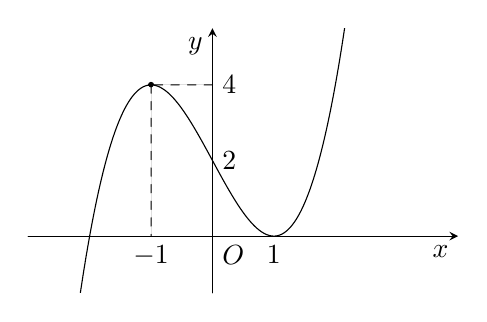
\begin{tikzpicture}[line join=round, line cap=round,>=stealth,y=0.8cm,x=1.3cm]
            \begin{scope}[scale=.6]
                \tikzset{label style/.style={font=\footnotesize}}
                \def \xmin{-3}
                \def \xmax{4}
                \def \ymin{-1.5}
                \def \ymax{5.5}
                \def \hamso{(\x)^3-3*(\x)+2}
                \draw[->] (\xmin,0)--(\xmax,0) node[below left] {$x$};
                \draw[->] (0,\ymin)--(0,\ymax) node[below left] {$y$};
                \draw (0,0) node [below right] {$O$};
                \clip (\xmin+0.01,\ymin+0.01) rectangle (\xmax-0.01,\ymax-0.01);
                \draw[samples=350,domain=\xmin+0.01:\xmax-0.01,smooth,variable=\x] plot (\x,{\hamso});
                \draw[dashed,fill] (0,4) node[right]{$4$}--(-1,4) circle (1.5pt)--(-1,0) node[below]{$-1$};
                \draw (1,0) node[below]{$1$} (0,2) node[right]{$2$};
            \end{scope}
        \end{tikzpicture}
    }
    \loigiai{\immini{$ g'(x)=f'(x)+2x-2 $. Cho $ g'(x)=0 \Leftrightarrow f'(x)=2-2x $.\\
            Vẽ đường thẳng $d \colon y=2-2x $. Đồ thị hàm số $ y=f'(x) $ cắt đường thẳng $ d $ tại $ 3 $ điểm có hoành độ lần lượt là $a$, $b$ và $c$.\\ Suy ra  phương trình $ g'(x)=0 $ có $ 3 $ nghiệm đơn $x=-1$, $x=0$, $x=1$.\\
            Bảng biến thiên
            \begin{center}
                \begin{tikzpicture}[scale=0.7]
                    \tkzTabInit[lgt=2,espcl=3.5]
                    {$x$/1.2,$g’(x)$/1.2,$g(x)$/2.5}
                    {$-\infty$,$-1$,$0$,$1$,$+\infty$}
                    \tkzTabLine{ ,-,0,+,0,-,0,+, }
                    \tkzTabVar{+/$ $,-/$ $,+/$ $,-/$ $,+/$ $}
                \end{tikzpicture}
            \end{center}
            Vậy hàm số $ y=g(x) $ có 1 điểm cực đại và 2 điểm cực tiểu.}
        {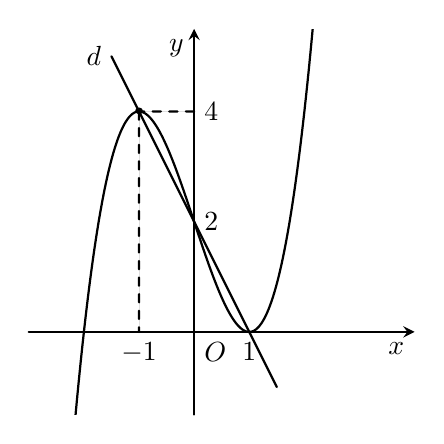
\begin{tikzpicture}[line join=round, line cap=round,>=stealth,thick,scale=0.7]
                \tikzset{label style/.style={font=\footnotesize}}
                \def \xmin{-3}
                \def \xmax{4}
                \def \ymin{-1.5}
                \def \ymax{5.5}
                \def \hamso{(\x)^3-3*(\x)+2}
                \draw[->] (\xmin,0)--(\xmax,0) node[below left] {$x$};
                \draw[->] (0,\ymin)--(0,\ymax) node[below left] {$y$};
                \draw (0,0) node [below right] {$O$};
                \begin{scope}
                    \clip (\xmin+0.01,\ymin+0.01) rectangle (\xmax-0.01,\ymax-0.01);
                    \draw[samples=350,domain=\xmin+0.01:\xmax-0.01,smooth,variable=\x] plot (\x,{\hamso});
                    \draw[dashed,fill] (0,4) node[right]{$4$}--(-1,4) circle (1.5pt)--(-1,0) node[below]{$-1$};
                    \draw (1,0) node[below]{$1$} (0,2) node[right]{$2$};
                \end{scope}
                \draw (-1.5,5) node[left]{$d$}--(1.5,-1);
        \end{tikzpicture}}
    }
\end{ex}
\begin{ex}%[2D1G2-2]

    Cho hàm số $y=f(x)$ có đồ thị như hình vẽ.
    Gọi $S$ là tập hợp tất cả các giá trị nguyên dương của tham số $m$ để đồ thị hàm số
    $y=\left|f\left(x-2019\right)+m\right|$ có 5 điểm cực trị. Tích giá trị các phần tử của $S$ bằng
    \begin{center}
        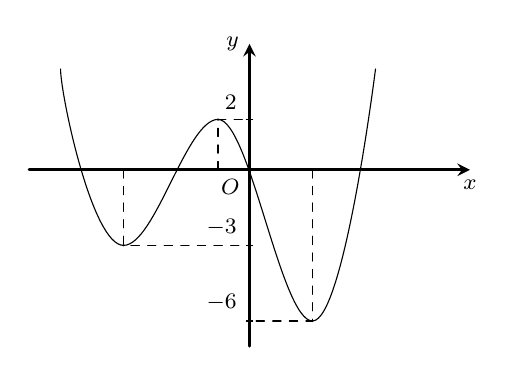
\begin{tikzpicture}[>=stealth,line join=round,line cap=round,font=\footnotesize,y=.8cm]
            \begin{scope}[scale=0.4]
                \def\xmin{-7} \def\xmax{7}
                \def\ymin{-7} \def\ymax{5}
                \draw[->,line width=1pt] (\xmin,0)--(\xmax,0) node [below]{$x$};
                \draw[->,line width=1pt] (0,\ymin)--(0,\ymax) node [left]{$y$};
                \node at (0,0) [below left]{$O$};
                %\fill (-2,0) node[below left]{$-2$};
                %\fill (1,0) node[below]{$1$};
                \draw
                (-6,4)
                .. controls + (90:-1) and + (180:1) .. (-4,-3)
                .. controls + (0:1) and + (180:1) .. (-1,2)
                .. controls + (0:1) and + (180:1) .. (2,-6)
                .. controls + (0:1) and + (0:0) .. (4,4)
                ;
                \foreach \x in {}\draw (\x,0.1)--(\x,-0.1) node[below right] {\footnotesize $\x$};
                \foreach \y in {-6,-3,2}\draw (0.1,\y)--(-0.1,\y) node [above left] {\footnotesize $\y$};
                \fill (0.0,0.0) circle (1pt);
                \draw[dashed] (2.0,0)--(2.0,-6.0)--(0,-6.0);\fill (2.0,-6.0) circle (1pt);
                \draw[dashed] (-1.0,0)--(-1.0,2.0)--(0,2.0);\fill (-1.0,2.0) circle (1pt);
                \draw[dashed] (-4.0,0)--(-4.0,-3.0)--(0,-3.0);\fill (-4.0,-3.0) circle (1pt);
            \end{scope}
        \end{tikzpicture}
    \end{center}
    \choice
    {$62$}
    {$56$}
    {\True $60$}
    {$60$}


    \loigiai{
        Đặt $g(x)=f\left(x-2019\right)+m$. Khi đó $g'(x)=f'\left(x-2019\right)$.\\
        Suy ra $$g'(x)=0\Leftrightarrow f'\left(x-2019\right)=0\Leftrightarrow\left[\begin{array}{*{20}{l}}
            {x-2019=x_1}\\
            {x-2019=x_2}\\
            {x-2019=x_3}
        \end{array}\right. \Leftrightarrow\left[\begin{array}{*{20}{l}}
            {x=2019+x_1}\\
            {x=2019+x_2}\\
            {x=2019+x_3,}
        \end{array}\right.$$
        với $x_1<x_2< 0 <x_3$.\\
        Bảng biến thiên
        \begin{center}
            \begin{tikzpicture}[scale=1, font=\footnotesize, line join=round, line cap=round, >=stealth]
                \tkzTab
                [lgt=1.5,espcl=3,]
                {$x$/1, $g’(x)$/1, $g(x)$/2.5}
                {$-\infty$, $2019+x_1$, $2019+x_2$,  $2019+x_3$, $+\infty$}
                {,-,0,+,0,-,0,+,}
                {}
                \draw
                (N12)node[below](A){$+\infty$}
                %(N13)node[above](A){ }
                ($(N22)!0.7!(N23)$)node(B){$m-3$}
                ($(N32)!0.4!(N33)$)node(C){$m+2$}
                %(N22)node[below](B){$g(-\tfrac{1}{2})$}
                %($(N32)!0.5!(N33)$)node(C){$g(\tfrac{1}{2})$}
                (N43)node[above](D){$m-6$}
                (N52)node[below](E){$+\infty$}
                ;
                \foreach \x/\y in {A/B,B/C,C/D,D/E}
                \draw[-stealth] (\x)--(\y);
            \end{tikzpicture}
        \end{center}
        Yêu cầu bài toán tương đương $\left[\begin{array}{*{20}{l}}
            {-6+m < 0\le-3+m}\\
            {m+2\le 0}
        \end{array}\right.$ $\Leftrightarrow\left[\begin{array}{*{20}{l}}
            {3\le m < 6}\\
            {m\le-2.}
        \end{array}\right.$\\
        Do đó $S=\left\{{3;\;4;\;5}\right\}$.\\
        Vậy tích các phần tử của $S$ là $3\cdot 4\cdot 5=60$.
    }
\end{ex}
\begin{ex}%[2D1G2-2]
    Cho hàm số $y=f\left(x\right)$ liên tục trên $\mathbb{R}$ có đồ thị như hình vẽ bên. Khi đó hàm số $g(x)=\left| f^2(x)-f(x)-12 \right|$ có bao nhiêu điểm cực trị?
    \begin{center}
        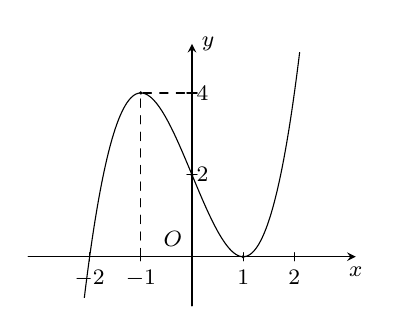
\begin{tikzpicture}[scale=.65, font=\footnotesize, line join=round, line cap=round, >=stealth,y=.8cm]
            \def\xmin{-3}\def\xmax{3}\def\ymin{-1}\def\ymax{5}
            \draw[->] (\xmin-0.2,0)--(\xmax+0.2,0) node[below] {\footnotesize $x$};
            \draw[->] (0,\ymin-0.2)--(0,\ymax+0.2) node[right] {\footnotesize $y$};
            \draw (0,0) node [above left] {\footnotesize $O$};
            \foreach \x in {-2,-1,1,2}\draw (\x,0.1)--(\x,-0.1) node [below] {\footnotesize $\x$};
            \foreach \y in {2,4}\draw (0.1,\y)--(-0.1,\y) node [right] {\footnotesize $\y$};
            \clip (\xmin,\ymin) rectangle (\xmax,\ymax);
            \draw[smooth,samples=200,domain=\xmin:\xmax] plot (\x,{1*((\x)^3)+0*((\x)^2)+-3*(\x)+2});
            \draw[dashed] (0.0,0)--(0.0,2.0)--(0,2.0);\fill (0.0,2.0) circle (1pt);
            \draw[dashed] (-1.0,0)--(-1.0,4.0)--(0,4.0);\fill (-1.0,4.0) circle (1pt);
            \draw[dashed] (1.0,0)--(1.0,0.0)--(0,0.0);\fill (1.0,0.0) circle (1pt);
        \end{tikzpicture}
    \end{center}
    \choice
    {\True $7$}
    {$9$}
    {$10$}
    {$8$}
    \loigiai{
        Xét hàm số $h(x)=f^2(x)-f(x)-12$.\\
        Đạo hàm $h'(x)=2.f(x).f'(x)-f'(x)$
        \\ $\bullet h'(x)=f'(x)\left[ 2.f(x)-1 \right]$
        \item $\bullet h'(x)=0\Leftrightarrow \left[ \begin{aligned}
            & f'(x)=0 \\
            & f(x)=\dfrac{1}{2} \\
        \end{aligned} \right.\Leftrightarrow \left[ \begin{aligned}
            & x=-1 \\
            & x=1 \\
            & x=x_1<-1 \\
            & x=x_2\in \left(0;1\right) \\
            & x=x_3>1 \\
        \end{aligned} \right.$.\\
        Dựa vào đồ thị hàm số $y=f\left(x\right)$ ta có: $h'(0)=f'(0)\left[ 2f(0)-1 \right]=f'(0)(2.2-1)<0$.\\
        $h(-1)=f^2(-1)-f(-1)-12=4^{2}-4-12=0$.\\
        $h(1)=f^2(1)-f(1)-12=-12$.\\
        Bảng biến thiên của hàm số $y=h\left(x\right)$
        \begin{center}
            
\begin{tikzpicture}[>=stealth]
                \tkzTabInit[nocadre=false,lgt=1,espcl=2,deltacl=0.6]{$x$/.7 ,$h'(x)$/1, $h(x)$/2}
                {$-\infty$ , $x_1$ , $-1$ , $x_2$, $1$, $x_3$ , $+\infty$}
                \tkzTabLine{ , - , $0$ , + , $0$ , - , $0$ , + , $0$ , - , $0$,+, }
                \tkzTabVar{+/$+\infty$ , -/, +/$0$ , -/$$ ,+/$-12$,-/$$, +/$+\infty$}
            \end{tikzpicture}
        \end{center}
        Hàm số $g(x)=|h(x)|$ có số điểm cực trị là số nghiệm đơn của phương trình $h'(x)=0$ và $h(x)=0$.
        \item Dựa theo BBT của $h(x)$ thì $g(x)$ có $7$ điểm cực trị.
    }
\end{ex}
\begin{ex}%[2D1G2-2]
    Cho hàm đa thức $y=f(x)$. Hàm số $y=f'(x)$ có đồ thị như hình vẽ bên. Có bao nhiêu giá trị của $m \in[0 ; 6]$; $2 m \in \mathbb{Z}$ để hàm số $g(x)=f\left(x^{2}-2|x-1|-2 x+m\right)$ có đúng $9$ điểm cực trị?
    \begin{center}
        \begin{tikzpicture}[scale=0.7, font=\footnotesize, line join=round, line cap=round, >=stealth,x=1.3cm,y=0.8cm]
            \draw[->] (-1,0) -- (0,0) node[below left]{$O$} -- (5,0) node[below]{$x$};
            \draw[->] (0,-2.5) -- (0,4) node[left]{$y$};
            \draw plot[domain=-0.5:3.1, samples=100] (\x,{-(\x)^2*(\x-1)*(\x-2)*(\x-3)});
            \draw (1,0) node[below]{$1$};
            \draw (2.2,0) node[below]{$2$};
            \draw (3.2,0) node[below]{$3$};
        \end{tikzpicture}
    \end{center}
    \choice
    {$7$}
    {$5$}
    {$3$}
    {\True $6$}
    \loigiai{
        Ta có $g(x)=f\left(x^{2}-2|x-1|-2 x+m\right)=f\left((x-1)^2-2|x-1|+m-1\right)$.\\
        Suy ra  $g(x)=f\left(|x-1|^2-2|x-1|+m-1\right)\Rightarrow g(x+1)=f\left(|x|^2 -2|x| +m -1\right)$.\\
        Ta có số điểm cực trị của $g(x)$ bằng số điểm cực trị của $g(x+1)$.\\
        Xét $h(x)=f\left(x^2-2x+m-1\right) \Rightarrow g(x+1)= h(|x|)$.\\
        Ta có $h'(x)=(2x-2)\cdot f'\left(x^2 -2x+m-1\right) = 0 \Leftrightarrow \hoac{&x =1 \\& f'\left(x^2-2x+m-1\right)=0.}$\\
        Ta thấy $f'(x)$ không đổi dấu khi $x$ qua $x=0$ nên ta chỉ cần xét\\
        \[f'\left(x^2-2x+m-1\right)=0  \Leftrightarrow \hoac{&x^2-2x+m-1 = 1\\&x^2-2x+m-1 = 2\\& x^2-2x+m-1 =3} \Leftrightarrow \hoac{&\left(x-1\right)^2=-m+3\\&\left(x-1\right)^2=-m+4\\&\left(x-1\right)^2=-m+5.}\]
        Ta có $g(x+1)$ có $9$ điểm cực trị khi $h(x)$ có $4$ điểm cực trị dương khi và chỉ khi \\
        $f'\left(x^2-2x+m-1\right)=0$ có $3$ nghiệm bội lẻ lớn hơn $0$, khác $1$ và các nghiệm còn lại là bội chẵn hoặc nhỏ hơn bằng $0$.\\
        Ta có bảng biến thiên của hàm số $y = (x-1)^2$
        \begin{center}
            
\begin{tikzpicture}[scale=1]
                \tkzTabInit[nocadre=false, lgt=1.2, espcl=2.5, deltacl=0.6]{$x$/0.6, $y$/2}{$-\infty$, $0$, $1$, $+\infty$}
                \tkzTabVar{+/$+\infty$, R, -/$0$, +/$+\infty$}
                \tkzTabVal{1}{3}{0.5}{}{$1$}
            \end{tikzpicture}
        \end{center}
        Từ bảng biến thiên ta có $\hoac{&0<-m+4 < 1\\&-m+3 \geq 1} \Leftrightarrow \hoac{&3<m<4 \\& m \leq 2}\Leftrightarrow \hoac{&6<2m<8\\&2m \leq 4.}$ \\
        Kết hợp với $m\in[0;6]$ và $2m\in\mathbb{Z}$, ta có $m \in\left\{0; \dfrac{1}{2}; 1; \dfrac{3}{2}; 2; \dfrac{7}{2}\right\}$.
    }
\end{ex}
\begin{ex}%[2D1G2-6]
    Cho hàm số $y=f(x)$ có đạo hàm, liên tục trên $\mathbb{R}$ và có đồ thị $y=f'(x)$ như hình vẽ. Hàm số $y=3f(x^2-2)+\dfrac{3}{2}x^4-3x^2$ đạt cực đại tại điểm nào sau đây?
    \begin{center}
        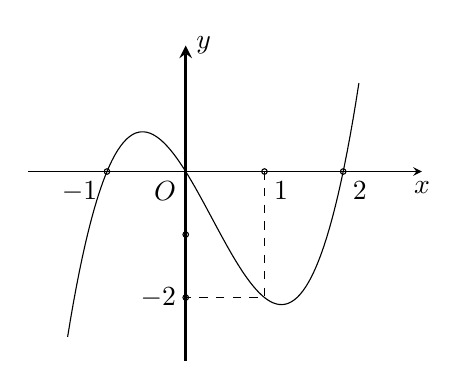
\begin{tikzpicture}[>=stealth,y=.8cm]
            \draw[->] (-2,0)--(0,0) node[below left]{$O$}--(3,0) node[below]{$x$};
            \draw[->,line width = 1pt] (0,-3) --(0,2) node[right]{$y$};
            \draw (-1,0) node[below left]{$-1$} circle (1pt);
            \draw (1,0) node[below right]{$1$} circle (1pt);
            \draw (2,0) node[below right]{$2$} circle (1pt);
            \draw (0,-2) node[left]{$-2$} circle (1pt);
            \draw (0,-1) circle (1pt);
            \draw [domain=-1.5:2.2, samples=100] %
            plot (\x, {(\x)^3-(\x)^2-2*(\x)});
            \draw [dashed] (1,0)--(1,-2)--(0,-2);
        \end{tikzpicture}
    \end{center}
    \choice
    {\True $x=0$}
    {$x=1$}
    {$x=-1$}
    {$x=2$}
    \loigiai{
        Đặt $g(x)=3f(x^2-2)+\dfrac{3}{2}x^4-3x^2 \Rightarrow g'(x)=3\cdot f(x^2-2)\cdot2x+6x^3-6x=6x\left[f'(x^2-2)+x^2-1\right]$.\\
        Suy ra $g'(x)=0\Leftrightarrow \hoac{&x=0\\&f'(x^2-2)=-x^2+1.}$\\
        Xét phương trình $f'(x^2-2)=-x^2+1$.\\
        Đặt $t=x^2-2 \Rightarrow -x^2+1=-t-1$ thì phương trình trở thành $f'(t)=-t-1$. Nghiệm của phương trình này là hoành độ giao điểm của đồ thị $y=f'(t)$ và đường thẳng $y=-t-1$.
        \begin{center}
            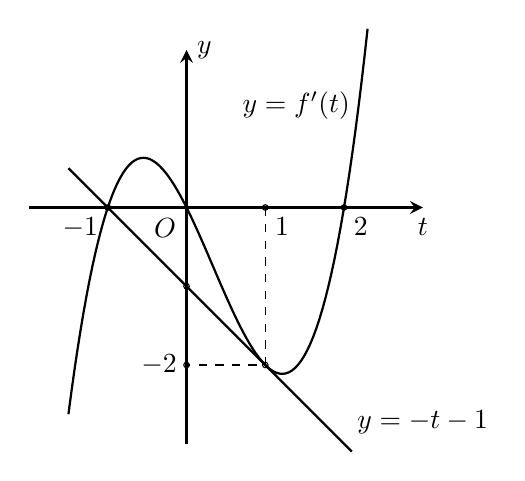
\begin{tikzpicture}[>=stealth]
                \draw[->,line width = 1pt] (-2,0)--(0,0) node[below left]{$O$}--(3,0) node[below]{$t$};
                \draw[->,line width = 1pt] (0,-3) --(0,2) node[right]{$y$};
                \draw (-1,0) node[below left]{$-1$} circle (1pt);
                \draw (1,0) node[below right]{$1$} circle (1pt);
                \draw (2,0) node[below right]{$2$} circle (1pt);
                \draw (0,-2) node[left]{$-2$} circle (1pt);
                \draw (0,-1) circle (1pt);
                \draw (1,-2) circle (1pt);
                \draw [thick, domain=-1.5:2.3, samples=100] %
                plot (\x, {(\x)^3-(\x)^2-2*(\x)});
                \draw [thick, domain=-1.5:2.1, samples=100] %
                plot (\x, {-(\x)-1});
                \draw [dashed] (1,0)--(1,-2)--(0,-2);
                \draw (2.2,1) node[above left]{$y=f'(t)$};
                \draw (3,-3) node[above]{$y=-t-1$};
            \end{tikzpicture}
        \end{center}
        Suy ra $f'(t)=-t-1\Rightarrow \hoac{&t=-1\\&t=1.}$\\
        \begin{itemize}
            \item $t=-1\Rightarrow x^2-2=-1\Leftrightarrow x=\pm1$.
            \item $t=1 \Rightarrow x^2-2=1\Leftrightarrow x=\pm\sqrt{3}$.
        \end{itemize}
        Từ đồ thị trên ta có
        \begin{itemize}
            \item $f'(t)+t+1>0\Leftrightarrow f'(t)>-t-1\Leftrightarrow \heva{&t>-1\\&t\neq1.}$\\
            Suy ra $\heva{&x^2-2>-1\\&x^2-2\neq1}\Leftrightarrow \heva{&x^2-1>0\\&x^2\neq3}\Leftrightarrow \heva{&x<-1\vee x>1\\&x\neq\sqrt{3}.}$
            \item $f'(t)+t+1>0\Leftrightarrow f'(t)>-t-1\Leftrightarrow t<-1$.\\
            Suy ra $x^2-2<-1\Leftrightarrow x^2-1<0\Leftrightarrow -1<x<1$.
        \end{itemize}
        Bảng biến thiên hàm số $y=g(x)$
        \begin{center}
            \begin{tikzpicture}
                \tkzTabInit[nocadre=false,lgt=4.5,espcl=1.8]
                {$x$ /1,$x$ /0.7,$f'(x^2-2)+x^2-1$ /0.7,$g'(x)$ /0.7,$g(x)$ /2}
                {$-\infty$,$-\sqrt{3}$,$-1$,$0$,$1$,$\sqrt{3}$,$+\infty$}
                \tkzTabLine{,-,|,-,|,-,$0$,+,|,+,|,+,}
                \tkzTabLine{,+,$0$,+,$0$,-,|,-,$0$,+,$0$,+,}
                \tkzTabLine{,-,$0$,-,$0$,+,$0$,-,$0$,+,$0$,+,}
                \tkzTabVar{+/,R,-/$y_\text{CT}$,+/$y_\text{CĐ}$,-/$y_\text{CT}$,R,+/}
            \end{tikzpicture}
        \end{center}
        Vậy hàm số đã cho đạt cực đại tại điểm $x=0$.
    }
\end{ex}
\begin{ex}%[2D1K2-6]
    Cho hàm số $f(x)=x^3-(2m-1)x^2+(2-m)x+2$. Tập hợp tất cả các giá trị thực của tham số $m$ để hàm số $y=f\left(\vert x\vert\right)$ có $5$ cực trị?
    \choice
    {$\dfrac{5}{4}\le m\le 2$}
    {$-\dfrac{5}{4}<m<2$}
    {$-2<m<\dfrac{5}{4}$}
    {\True $\dfrac{5}{4}<m<2$}
    \loigiai{
        Tập xác định $\mathscr{D}=\mathbb{R}$.\\
        Ta có $f\left(|-x|\right)=f\left(|x|\right)$, $\forall x\in\mathbb{R}$ nên $y=f\left(|x|\right)$ là hàm số chẵn. \\
        Do đó, đồ thị hàm số $y=f\left(|x|\right)$ đối xứng qua trục tung.\\
        Suy ra hàm số $y=f\left(|x|\right)$ luôn có một điểm cực trị là $x=0$.\\
        Do đó, $y=f\left(|x|\right)$ có $5$ điểm cực trị $\Leftrightarrow$ hàm số $y=f(x)$ có $2$ điểm cực trị dương.\\
        \phantom{Do đó, số $y=f\left(|x|\right)$ có $5$ điểm cực trị} $\Leftrightarrow$ $f'(x)=0$ có hai nghiệm dương phân biệt.\\
        Ta có $f'(x)=3x^2-2(m-1)x+2-m$.\\
        Yêu cầu bài toán $\Leftrightarrow\heva{&\Delta'>0 \\ &S>0 \\ &P>0}\Leftrightarrow\heva{&4m^2-m-5>0 \\ &2m-1>0 \\ &2-m>0}\Leftrightarrow\heva{&m<-1\;\text{hoặc}\;m>\dfrac{5}{4} \\ &m>\dfrac{1}{2} \\ &m<3}\Leftrightarrow \dfrac{5}{4}<m<2$.
    }
\end{ex}
\Closesolutionfile{ans}
%% \indapan{10}{ans/2D1-2-DEON-1}